\documentclass[a4paper,10pt]{article}
\usepackage[utf8]{inputenc}
\usepackage{amsmath}
\usepackage{graphicx}
\numberwithin{equation}{section}
%opening
\title{Math Phys II HW 2}
\author{Vince Baker}

%opening
\title{}
\author{Vince Baker}

\begin{document}

\maketitle

\begin{abstract}

\end{abstract}

\section{Problem 1}
We solve the harmonic oscillator by writing down the classical Hamiltonian, replacing the momentum by $\frac{\hbar}{i}\frac{d}{dx}$, and solving.
The classical Hamiltonian is:
\begin{equation}
H=\frac{p^2}{2m}+\frac{1}{2}kx^2
\end{equation}
Replacing p with $\frac{\hbar}{i}\frac{d}{dx}$:
\begin{gather}
\{ \frac{-\hbar ^2}{2m}\frac{d^2}{dx ^2}+\frac{1}{2}kx^2\}\Psi=E\Psi\\
\frac{d^2 \Psi}{dx^2}-\frac{mkx^2}{\hbar ^2}\Psi+\frac{2mE}{\hbar^2}\Psi=0
\end{gather}
We now make a transformation $x=\gamma z$ into dimensionaless coordinates.
\begin{gather}
\frac{1}{\gamma ^2}\frac{d^2 \Psi}{dz^2}-\frac{mk}{\hbar ^2}\gamma^2z^2\Psi+\frac{2mE}{\hbar^2}\Psi=0\\ 
\frac{d^2 \Psi}{dz^2}-\frac{mk}{\hbar ^2}\gamma^4z^2\Psi+\frac{2mE}{\hbar^2}\Psi=0\\ 
\end{gather}
Table 22.6 of A\&S has the solution for this general form, with the coefficient of the z term $2n+1-x^2$.
The solutions are $e^{\frac{-x^2}{2}}H_n(x)$ with $H_n(x)$ the Hermite polynomials. 
Solving for the dimensionless parameter $\gamma$ we find:
\begin{gather}
\frac{mk}{\hbar ^2} \gamma ^4=1\\
\gamma ^2=\frac{\hbar }{\sqrt{mk}}\\
\frac{2mE}{\hbar ^2}\gamma ^2=2n+1\\
E=\frac{\hbar ^2}{2m}\frac{\sqrt{mk}}{\hbar}(2n+1)=\hbar \sqrt{\frac{k}{m}}(n+\frac{1}{2})
\end{gather}
We plot the analytic solutions for the 1-D quantum harmonic oscillator. 
\begin{equation}
 \Psi(x)_n=\frac{1}{\sqrt{2^n n! \sqrt{\pi}}}H_n(x)
\end{equation}
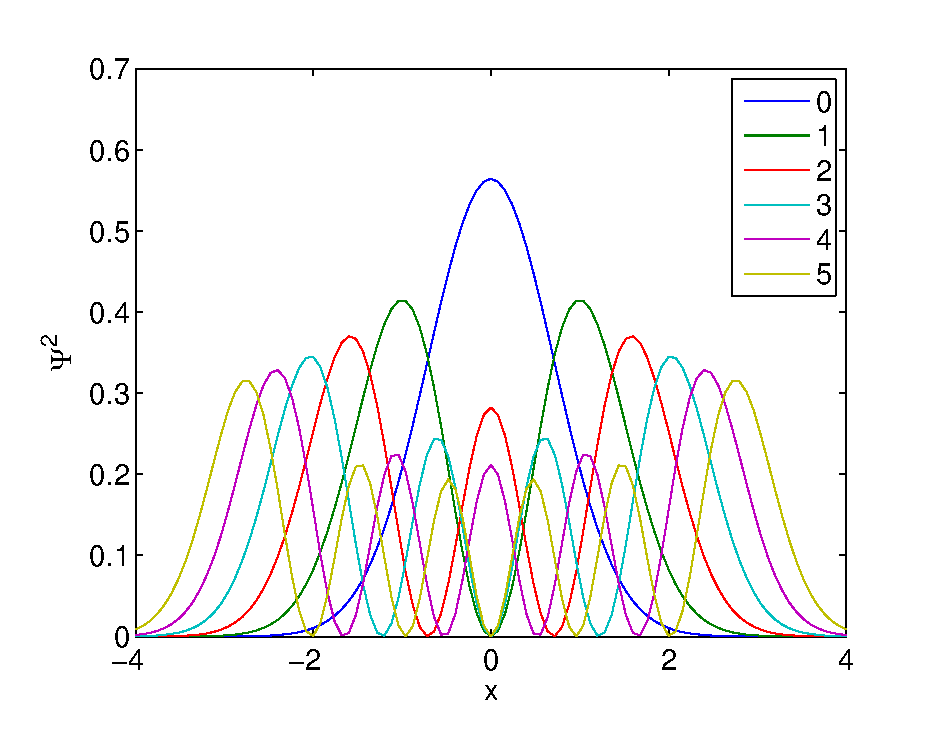
\includegraphics{analytic}
\linebreak
We then approximate the solution using a numerical estimate of the second derivative. 
The 6 lowest eigenvalues are (to within .01) 0.5, 1.5, 2.5, 3.5, 4.5 and 5.5 in close agreement with the analytical energy levels $n+\frac{1}{2}$. 
Increasing the number of lattice sites from 101 to 1001 improves the agreement to .001.
\end{document}
